%==============================================================================
% PSI5120 - Final Assignment
% Extending a Comparative Study of Kubernetes HPA: statistical variability,
% node-level saturation, and autoscaling beyond CPU.
%
% Template: IEEEtran (two columns). Compile on Overleaf or:
%   pdflatex artigo.tex  (run twice to resolve references)
%
% Figures expected in ./figuras/ (names match the \includegraphics below).
%==============================================================================
\documentclass[conference]{IEEEtran}
\IEEEoverridecommandlockouts

\usepackage[utf8]{inputenc}
\usepackage[T1]{fontenc}
\usepackage[english]{babel}
\usepackage{graphicx}
\usepackage{booktabs}
\usepackage{listings}
\usepackage{xcolor}
\usepackage{url}
\usepackage{amsmath}
\usepackage{tikz}
\usetikzlibrary{positioning,fit,backgrounds}

\lstset{
  basicstyle=\ttfamily\footnotesize,
  breaklines=true,
  frame=single,
  captionpos=b,
  columns=fullflexible,
  keepspaces=true,
  showstringspaces=false
}

\begin{document}

\title{Extending a Comparative Study of Kubernetes Horizontal Pod Autoscaling:\\
Statistical Variability, Node-Level Saturation, and Metrics Beyond CPU}

\author{\IEEEauthorblockN{Vitor Augusto Takeuchi}
\IEEEauthorblockA{Escola Politécnica --- University of São Paulo\\
PSI5120 --- Topics in Cloud Computing\\
NUSP: 11327606}}

\maketitle

%------------------------------------------------------------------------------
\begin{abstract}
This work extends a previous comparative study of the Kubernetes Horizontal Pod
Autoscaler (HPA) between a local cluster (Minikube) and a managed cloud cluster
(Amazon EKS). The prior study concluded that the same declarative manifests
produce equivalent scaling behaviour in both environments, but it explicitly
listed three limitations: it relied on a single execution, it did not evaluate
cluster saturation or node-level scaling, and it considered CPU as the only
scaling metric. Here we address each limitation through controlled experiments
run entirely on Minikube, at no cloud cost. First, we repeat the CPU-based
experiment ten times and report the run-to-run variability, showing that
single-run figures should not be read as constants: the time to the first
scaling action varied by roughly 23\% and the sampled CPU peak by roughly 25\%
around their means. Second, on a three-node local cluster we reproduce Pod
distribution across nodes and, by exceeding the aggregate capacity, we observe
Pods stuck in the \texttt{Pending} state, confirming that the HPA controls the
desired number of replicas but does not create capacity. Third, we drive the HPA
by memory instead of CPU and show that the same mechanism scales on a different
signal, with a qualitatively different dynamic. Together, the extensions
strengthen the interpretation of the original results and clarify the boundary
between workload autoscaling and infrastructure scaling.
\end{abstract}

\begin{IEEEkeywords}
Kubernetes, autoscaling, HPA, cloud computing, Minikube, statistical
variability, cluster saturation, custom metrics.
\end{IEEEkeywords}

%==============================================================================
\section{Introduction}
%==============================================================================
Elasticity --- adjusting computational resources to match demand --- is a central
property of cloud computing~\cite{catillo2022,galante2012}. In containerized
environments consolidated by container technologies~\cite{bernstein2014} and
orchestrators such as Kubernetes~\cite{burns2016}, one way to realize elasticity
is the Horizontal Pod Autoscaler (HPA)~\cite{k8s-hpa-doc,nguyen2020}, which
adjusts the number of replicas of an application from observed metrics, commonly
CPU utilization.

In a previous assignment we compared the HPA behaviour between a local Minikube
cluster and a managed Amazon EKS cluster, using identical manifests. The main
finding was that the logical scaling behaviour was equivalent in both
environments (both scaled from 1 to 6 replicas under the same load and returned
to the minimum afterwards), while the relevant differences appeared in topology,
metric provisioning, cost, and management effort. That study, however, closed
with three explicit limitations:

\begin{enumerate}
  \item results came from a \emph{single execution}, with no repetition or
        statistical treatment;
  \item it did \emph{not} evaluate what happens when the cluster runs out of
        capacity, nor node-level scaling;
  \item it used \emph{only CPU} as the scaling metric, noting that CPU may not
        reflect the full demand of an application.
\end{enumerate}

This paper takes those three limitations as its agenda. Each is addressed by a
dedicated experiment, and --- following the restriction of avoiding further cloud
cost --- all new experiments run on Minikube. The managed-cloud results from the
prior work are reused as an already-measured baseline. All code, manifests, and
evidence are publicly available at
\url{https://github.com/VitorTakeuchi/psi5120-hpa}.

The remainder of the paper is organized as follows. Section~\ref{sec:bg} reviews
the background; Section~\ref{sec:rel} discusses related work;
Section~\ref{sec:baseline} summarizes the baseline (the intermediate study);
Sections~\ref{sec:ext1}, \ref{sec:ext2} and~\ref{sec:ext3} present the three
extensions; Section~\ref{sec:disc} discusses the combined findings; and
Section~\ref{sec:conc} concludes.

%==============================================================================
\section{Background}
\label{sec:bg}
%==============================================================================
A \emph{Pod} is the smallest deployable unit in Kubernetes and wraps one or more
containers. A \emph{Deployment} manages the lifecycle of a set of identical Pods,
maintaining the desired replica count. A \emph{Service} provides a stable access
point that distributes requests among the active replicas.

The HPA periodically computes the desired number of replicas by comparing an
observed metric with a target value. It can be understood as a feedback
controller: the observed metric is the input signal, the target is the reference,
and the replica count is the controlled variable~\cite{nguyen2020}. For CPU
utilization, the desired replica count follows~\cite{k8s-hpa-doc}:
\begin{equation}
r_{desired} = \left\lceil r_{current} \times
\frac{U_{current}}{U_{target}} \right\rceil
\label{eq:hpa}
\end{equation}
where $r$ is the replica count and $U$ the CPU utilization as a percentage of the
Pod's \texttt{requests}. The ceiling operator explains why the HPA may keep an
extra replica even when utilization is close to the target. CPU metrics are
provided by the \emph{Metrics Server}, which exposes recent resource-usage
metrics through the Metrics API~\cite{metrics-server}; without it the HPA reports
the metric as \texttt{<unknown>}.

%==============================================================================
\section{Related Work}
\label{sec:rel}
%==============================================================================
Autoscaling in the cloud has been widely studied. Broad surveys describe
elasticity as a central property of cloud computing and classify scaling policies
as reactive/proactive and horizontal/vertical, discussing over- and
under-provisioning~\cite{catillo2022,galante2012,lorido2014}. Within Kubernetes,
recent surveys place the HPA as only one of several elasticity layers, alongside
the Vertical Pod Autoscaler (VPA), which adjusts per-instance resources, and the
Cluster Autoscaler, which changes the number of worker
nodes~\cite{survey-k8s-2022,aggarwal2025}.

Experimentally, Nguyen et al.~\cite{nguyen2020} evaluate the HPA across multiple
runs, analysing CPU utilization, replica count, request failures and, notably,
the influence of the metric-collection interval on the reaction time. They stress
that metric refresh, Pod creation and application start-up all affect the scaling
dynamics, and that CPU-only metrics may not capture the full application demand.
The present work is aligned with these observations: rather than proposing a new
algorithm, it evaluates, in a controlled way, the \emph{behavioural portability}
and the \emph{operational boundaries} of the HPA, extending a local-vs-managed
comparison with repeated trials, saturation, and an alternative metric.

%==============================================================================
\section{Baseline: the intermediate study}
\label{sec:baseline}
%==============================================================================
The baseline deploys the same three Kubernetes objects in both environments: a
\texttt{Deployment} of a CPU-bound web server (image
\texttt{registry.k8s.io/hpa-example}, the one used in the official HPA
walkthrough~\cite{k8s-hpa}), a \texttt{ClusterIP} \texttt{Service}, and an HPA
with \texttt{minReplicas=1}, \texttt{maxReplicas=10} and a target of 50\% average
CPU utilization. Load was generated by a \texttt{busybox} Pod issuing HTTP
requests in a loop; metrics were sampled every 5\,s.

Table~\ref{tab:baseline} summarizes the baseline results. In both environments
the HPA scaled from 1 to 6 replicas under load and returned to 1 after the load
stopped, following the 300\,s scale-down stabilization window. The essential
difference was topological: on Minikube (single node) all replicas shared one
machine, whereas on EKS (two nodes across two availability zones) the replicas
were distributed across nodes. This baseline is reused here as the reference
point; the extensions below investigate what it did not cover.

\begin{table}[!t]
\caption{Baseline results (intermediate study): Minikube vs.\ Amazon EKS,
single run.}
\label{tab:baseline}
\centering
\begin{tabular}{@{}lcc@{}}
\toprule
\textbf{Metric} & \textbf{Minikube} & \textbf{Amazon EKS} \\
\midrule
Nodes                    & 1        & 2 (\texttt{t3.small}) \\
Sampled CPU peak         & 228\%    & 244\%    \\
Max replicas             & 6        & 6        \\
Scale up (1$\to$6)       & $\approx$4 min & $\approx$4 min \\
Scale down ($\to$1)      & $\approx$5 min & $\approx$5 min \\
Pod distribution         & single node & 2 nodes \\
\bottomrule
\end{tabular}
\end{table}

Figs.~\ref{fig:base-mk} and~\ref{fig:base-eks} show the baseline replica and CPU
curves for Minikube and EKS, respectively. In both, the CPU utilization overshoots
sharply at the onset of load, the replica count rises in discrete steps, and the
average utilization then converges towards the 50\% target as new replicas absorb
the load. The curves are qualitatively identical, which is the visual basis for
the baseline's central claim of behavioural portability.

\begin{figure}[!t]
\centering
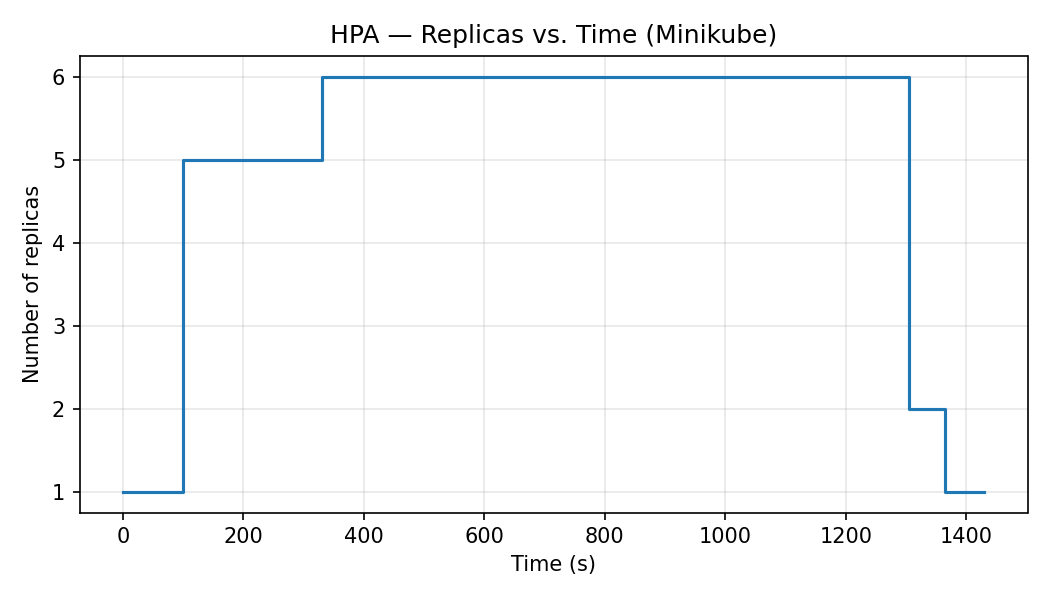
\includegraphics[width=\columnwidth]{figuras/baseline_minikube_replicas.png}\\[2pt]
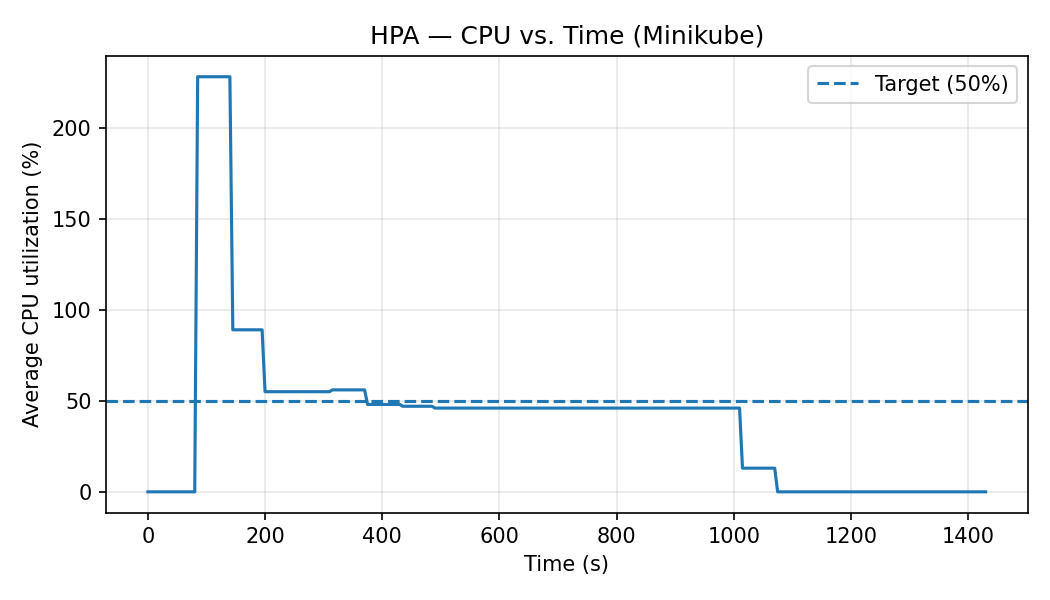
\includegraphics[width=\columnwidth]{figuras/baseline_minikube_cpu.png}
\caption{Baseline (Minikube): replicas over time (top) and average CPU
utilization with the 50\% target (bottom).}
\label{fig:base-mk}
\end{figure}

\begin{figure}[!t]
\centering
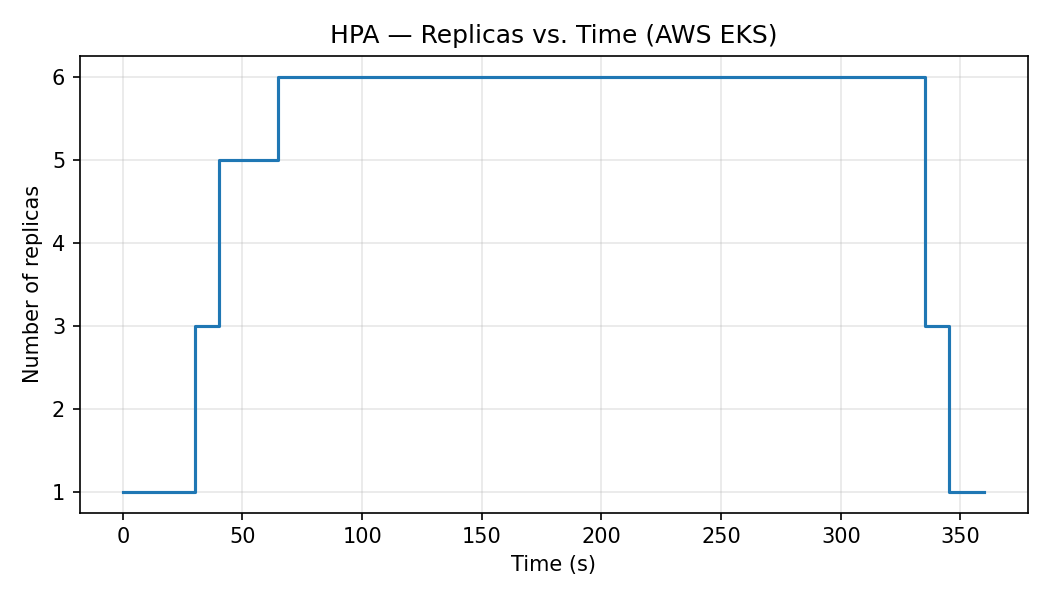
\includegraphics[width=\columnwidth]{figuras/baseline_eks_replicas.png}\\[2pt]
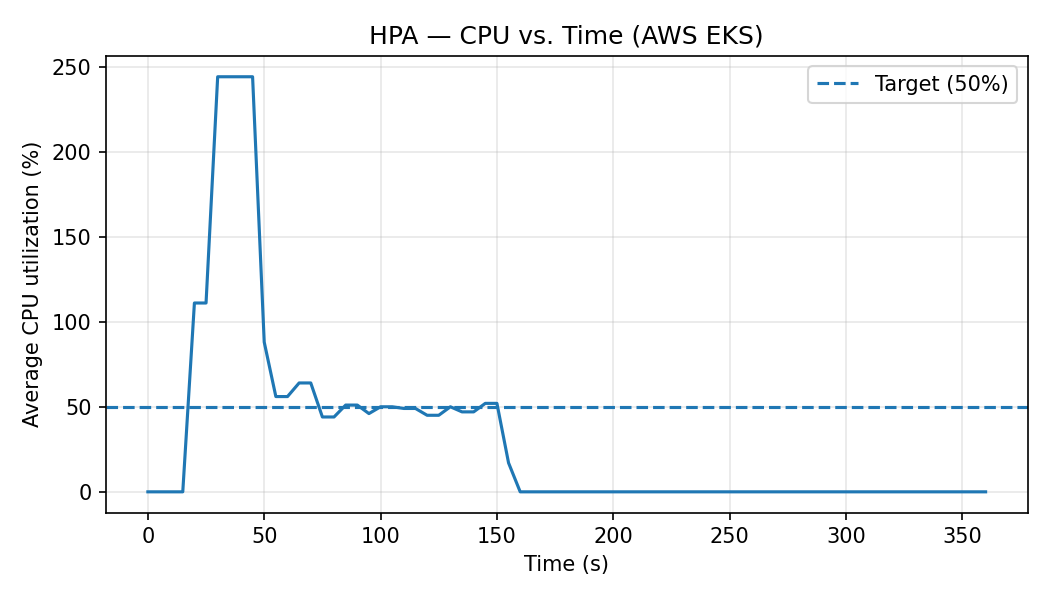
\includegraphics[width=\columnwidth]{figuras/baseline_eks_cpu.png}
\caption{Baseline (Amazon EKS): replicas over time (top) and average CPU
utilization with the 50\% target (bottom).}
\label{fig:base-eks}
\end{figure}

\subsection{Experimental setup}
\label{sec:setup}
All new experiments were executed on a single physical machine (Ubuntu~24.04,
x86\_64) using Minikube with the Docker driver. Table~\ref{tab:setup} records the
versions and per-experiment parameters, so that the results can be reproduced and
so that the discrete metric-collection interval --- a known influence on the
measured reaction time~\cite{nguyen2020} --- is explicit. Minikube runs
Kubernetes~1.35.1 with the Metrics Server~0.8.1 addon; the managed baseline used
Amazon EKS with Kubernetes~1.33. The metric-collection interval of the helper
script (5\,s) is an observation cadence and should not be confused with the
internal refresh interval of the Metrics Server or the HPA sync period; the
sampled values reported here are therefore lower bounds on instantaneous peaks.

\begin{table}[!t]
\caption{Experimental setup and per-experiment parameters.}
\label{tab:setup}
\centering
\begin{tabular}{@{}lp{0.52\columnwidth}@{}}
\toprule
\textbf{Item} & \textbf{Value} \\
\midrule
Host OS            & Ubuntu 24.04 (x86\_64) \\
Minikube / driver  & 1.38.1 / Docker 29.2.1 \\
Kubernetes (local) & 1.35.1 \\
Metrics Server     & 0.8.1 \\
Sampling interval  & 5\,s \\
HPA API            & \texttt{autoscaling/v2} \\
\midrule
\multicolumn{2}{@{}l}{\textit{E1 --- repeated trials}} \\
\quad Trials ($N$)         & 10 \\
\quad Load window          & 180\,s + cool-down \\
\quad requests / target    & cpu 200\,m / 50\% \\
\midrule
\multicolumn{2}{@{}l}{\textit{E2 --- saturation}} \\
\quad Nodes                & 3 (1 control-plane, 2 workers; 2\,vCPU each) \\
\quad requests / maxReplicas & cpu 500\,m / 30 \\
\midrule
\multicolumn{2}{@{}l}{\textit{E3 --- memory}} \\
\quad Image / requests     & \texttt{polinux/stress} / mem 150\,Mi \\
\quad Target / alloc       & memory 60\% / $\approx$120\,Mi per Pod \\
\bottomrule
\end{tabular}
\end{table}

%==============================================================================
\section{Extension 1: Repeated Trials and Statistical Variability}
\label{sec:ext1}
%==============================================================================
\subsection{Method}
To address the single-execution limitation, the CPU-based experiment was repeated
$N=10$ times on the single-node Minikube cluster. Each trial applied a fixed
180\,s load window followed by a cool-down, and a helper script recorded, every
5\,s, the replica count and the CPU utilization reported by the HPA. For each
trial we extracted three metrics: the time to the first scaling action, the
maximum replica count, and the sampled CPU peak. The ten trials were then
aggregated into mean and standard deviation.

\subsection{Results}
Table~\ref{tab:ext1} reports the aggregated results. The dispersion is
substantial: the time to the first scaling action varied by about 23\% of its
mean, and the sampled CPU peak by about 25\%. The maximum replica count was not
constant either (mean $4.6$, standard deviation $0.84$), i.e.\ different runs
under nominally identical conditions reached different peak replica counts.

\begin{table}[!t]
\caption{Extension 1 --- ten repeated trials on Minikube (mean $\pm$ std).}
\label{tab:ext1}
\centering
\begin{tabular}{@{}lc@{}}
\toprule
\textbf{Metric} & \textbf{Mean $\pm$ Std} \\
\midrule
Time to first scaling (s) & $72.9 \pm 17.1$ \\
Maximum replicas          & $4.6 \pm 0.84$  \\
Sampled CPU peak (\%)     & $196.4 \pm 48.6$ \\
\bottomrule
\end{tabular}
\end{table}

Fig.~\ref{fig:ext1} shows the replica count over time for all ten trials (grey),
with the mean (solid) and the $\pm 1$ standard-deviation band (shaded). The band
is widest during the scale-up transient, which is precisely where the reaction
time varies most.

\begin{figure}[!t]
\centering
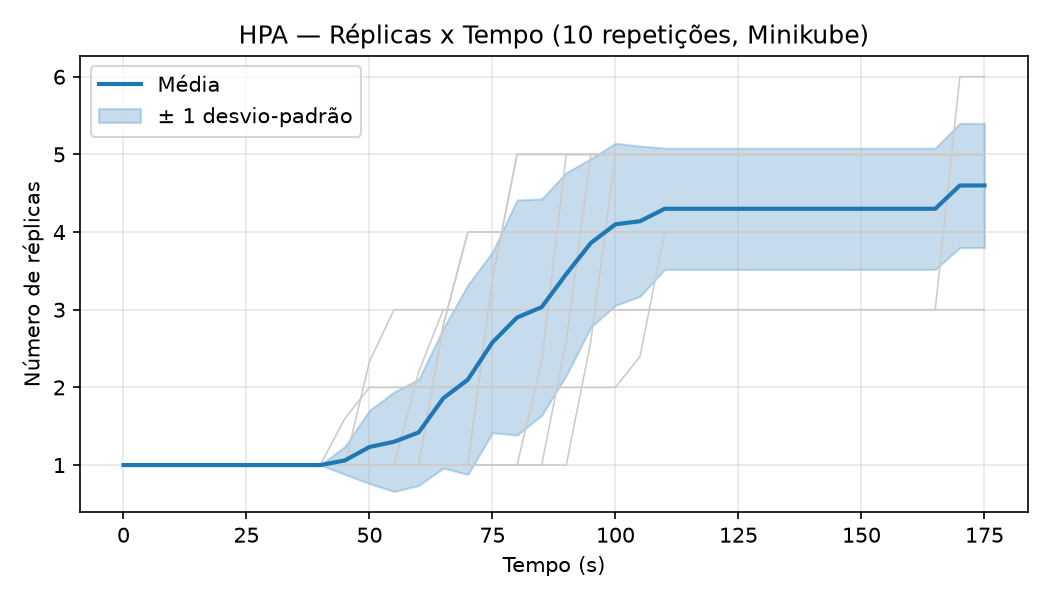
\includegraphics[width=\columnwidth]{figuras/ext1_replicas_media_desvio.png}
\caption{Extension 1: replicas over time across ten trials (grey), with mean and
$\pm 1$ standard-deviation band. The variability is concentrated in the scale-up
transient.}
\label{fig:ext1}
\end{figure}

\subsection{Interpretation}
This result directly qualifies the baseline. The single-run baseline reported
``228\% and 6 replicas'' as if they were fixed; the repeated trials show that
such values are samples of a distribution with non-negligible spread. Expressed as
a coefficient of variation (std/mean), the dispersion is about 23\% for the time
to first scaling and 25\% for the sampled CPU peak --- large enough that two
single runs could easily differ by tens of percent for reasons unrelated to the
environment. In particular, the baseline's Minikube-vs-EKS CPU peaks (228\% vs.\
244\%, a 7\% difference) fall comfortably inside this one-environment spread,
which means that difference cannot be attributed to the platform.
Two sources plausibly explain the spread: the discrete 5\,s sampling (a true peak
may fall between samples) and the chain of events behind each scaling decision
(metric refresh, Pod scheduling, container start-up), whose timing fluctuates. The
maximum replica count here (mean $4.6$) is lower than the baseline's 6; this is
attributable to the shorter, fixed 180\,s load window used to keep the ten trials
comparable, rather than to a different mechanism. The methodological takeaway is
that reaction time and peak values should be reported as distributions, not as
constants --- consistent with prior experimental work~\cite{nguyen2020}, which
repeats each scenario multiple times for exactly this reason.

%==============================================================================
\section{Extension 2: Node-Level Elasticity and Saturation}
\label{sec:ext2}
%==============================================================================
\subsection{Method}
To address the capacity/node limitation, a three-node Minikube cluster was
created (one control-plane node and two workers), each node deliberately small
(2~vCPU). The web server was deployed with larger CPU \texttt{requests} (500\,m
per Pod) and the HPA \texttt{maxReplicas} was raised to 30, so that the demanded
replica count could exceed the cluster's aggregate capacity.
Fig.~\ref{fig:ext2-nodes} shows the three nodes in the \texttt{Ready} state. The
deployment and HPA differ from the baseline only in their sizing, shown in
Listing~\ref{lst:hpa-sat}: larger CPU requests and a higher replica ceiling, so
the demanded count can outgrow the cluster.

\begin{lstlisting}[language=,caption={Extension 2: deployment sizing and HPA that
can exceed cluster capacity (excerpt).},label=lst:hpa-sat]
# deployment: larger requests -> saturates sooner
resources:
  requests:
    cpu: 500m        # vs 200m in the baseline
# hpa: higher ceiling than the cluster can run
spec:
  minReplicas: 1
  maxReplicas: 30    # exceeds aggregate capacity
  metrics:
  - type: Resource
    resource: {name: cpu, target: {type: Utilization, averageUtilization: 50}}
\end{lstlisting}

\begin{figure}[!t]
\centering
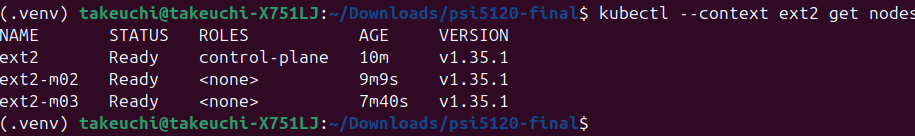
\includegraphics[width=\columnwidth]{figuras/ext2_nodes.png}
\caption{Extension 2: local three-node cluster (\texttt{kubectl get nodes}), one
control-plane node and two workers.}
\label{fig:ext2-nodes}
\end{figure}

\subsection{Results: distribution and saturation}
Under load, the scheduler distributed the running replicas across the three nodes
(Fig.~\ref{fig:ext2-dist}), reproducing locally --- and at no cost --- the
multi-node distribution observed on EKS in the baseline. The same figure already
shows several Pods in the \texttt{Pending} state with no assigned node, i.e.\ the
scheduler could not place them.

\begin{figure}[!t]
\centering
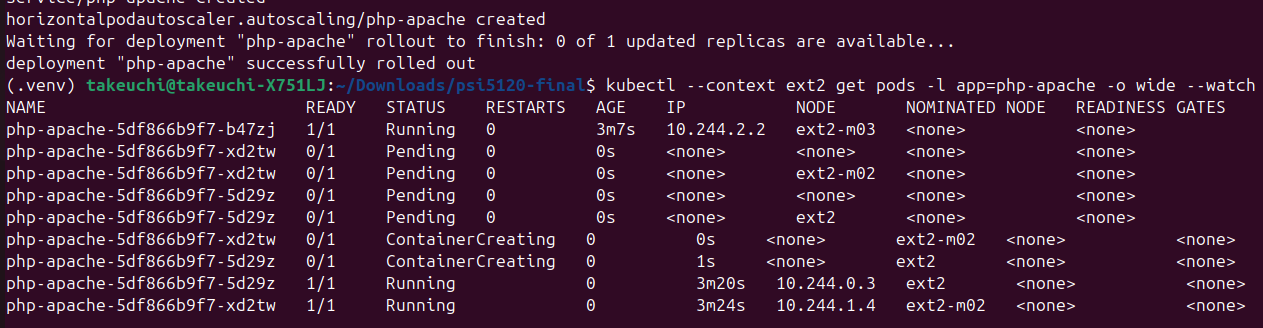
\includegraphics[width=\columnwidth]{figuras/ext2_distribuicao_pending.png}
\caption{Extension 2: running replicas distributed across the three nodes, with
additional Pods held in \texttt{Pending} (no node assigned) at the peak.}
\label{fig:ext2-dist}
\end{figure}

Under the applied (single-generator) load, the HPA settled at three running
replicas with CPU around 54\%/50\% (Fig.~\ref{fig:ext2-hpa}); with 500\,m
requests on small nodes, that was as far as this load drove the desired count.
To probe the capacity ceiling directly, the replica count was then raised
manually to 40. The cluster could only run a fraction of them, as
Listing~\ref{lst:ready} shows: 15 replicas \texttt{READY} out of 40 requested,
the remaining Pods rejected by the scheduler for insufficient CPU.

\begin{figure}[!t]
\centering
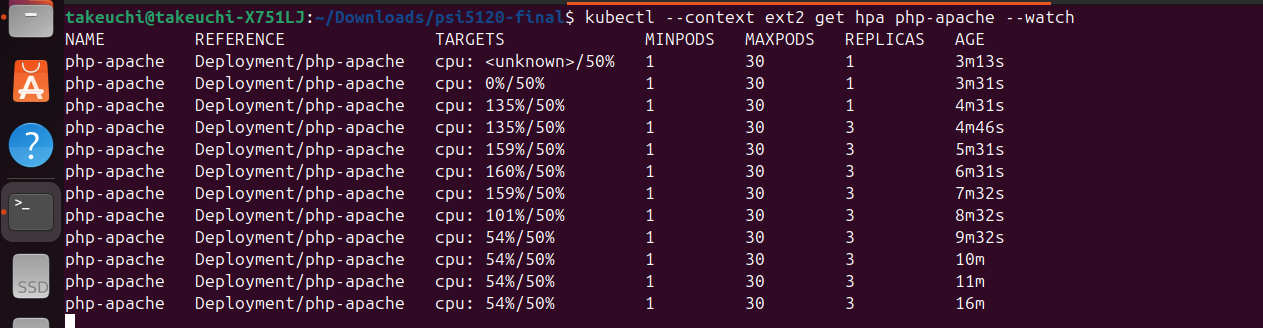
\includegraphics[width=\columnwidth]{figuras/ext2_watch_hpa.png}
\caption{Extension 2: HPA under load on the three-node cluster; the desired
replica count stabilizes at three given the applied load.}
\label{fig:ext2-hpa}
\end{figure}

\begin{lstlisting}[caption={Saturation: 15 of 40 requested replicas are Ready;
the rest cannot be scheduled for lack of CPU.},label=lst:ready]
$ kubectl get deployment php-apache
NAME         READY   UP-TO-DATE   AVAILABLE   AGE
php-apache   15/40   40           15          20m
\end{lstlisting}

\subsection{Interpretation}
This experiment makes concrete a conceptual boundary of the HPA. The HPA decides
\emph{how many} replicas should exist, but it does not create worker capacity: a
Deployment can request 40 replicas while the cluster runs only 15. Placing each
Pod on a node is the scheduler's responsibility, based on available resources and
scheduling constraints~\cite{k8s-topology}; therefore the node distribution
observed above is an outcome of the scheduler, not an intrinsic behaviour of the
HPA. When aggregate capacity is exhausted, raising \texttt{maxReplicas} does not
help: elasticity at the infrastructure level requires a separate mechanism such
as the Cluster Autoscaler or Karpenter~\cite{aws-autoscaling,survey-k8s-2022}.
The baseline could not show this because it never approached saturation.

%==============================================================================
\section{Extension 3: Autoscaling Beyond CPU}
\label{sec:ext3}
%==============================================================================
\subsection{Method}
To address the single-metric limitation, the HPA was driven by \emph{memory}
instead of CPU, using the same \texttt{autoscaling/v2} API --- only the
\texttt{resource.name} field changes, with a 60\% memory-utilization target
(Listing~\ref{lst:hpa-mem}). A memory-consuming application
(\texttt{polinux/stress}) was deployed with \texttt{requests.memory=150Mi}, each
replica allocating roughly 120\,Mi.

\begin{lstlisting}[language=,caption={Extension 3: the only change from a CPU-based
HPA is the metric name and target (excerpt).},label=lst:hpa-mem]
metrics:
- type: Resource
  resource:
    name: memory     # <- was cpu
    target:
      type: Utilization
      averageUtilization: 60
\end{lstlisting}

\subsection{Results}
Fig.~\ref{fig:ext3-hpa} shows the HPA scaling on memory: as utilization exceeded
the 60\% target, the replica count grew from 1 to 4. Notably, memory utilization
remained pinned at 80\%/60\% and did \emph{not} converge to the target the way
CPU did in the baseline. Fig.~\ref{fig:ext3-top} explains why: each replica holds
about 120\,Mi and reports essentially 0\,m of CPU. Because the \texttt{stress}
workload never releases the memory it allocates, adding replicas does not dilute
the per-replica average as happens with CPU.

\begin{figure}[!t]
\centering
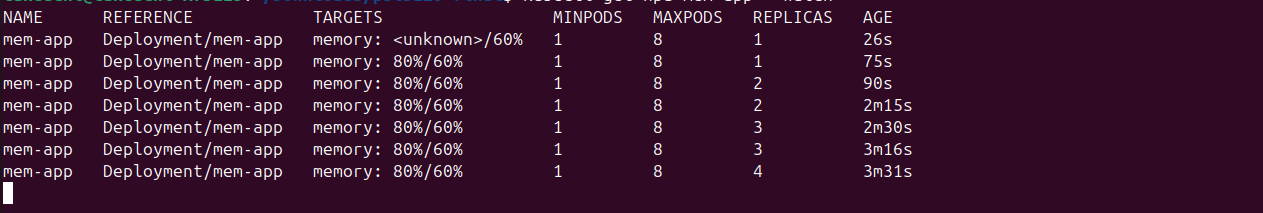
\includegraphics[width=\columnwidth]{figuras/ext3_hpa_memoria.png}
\caption{Extension 3: HPA driven by memory (\texttt{memory: 80\%/60\%}); the
replica count grows from 1 to 4.}
\label{fig:ext3-hpa}
\end{figure}

\begin{figure}[!t]
\centering

\includegraphics[width=\columnwidth]{figuras/ext3_top_pods.png}
\caption{Extension 3: per-Pod usage (\texttt{kubectl top pods}); about 120\,Mi of
memory each and near-zero CPU.}
\label{fig:ext3-top}
\end{figure}

\subsection{Interpretation}
Two points follow. First, the same mechanism scales on a different signal with no
architectural change, confirming that the choice of metric --- not the HPA
itself --- determines what "demand" means. In fact, with CPU near 0\,m, this
workload would never scale under a CPU-based policy but scales readily under a
memory-based one. Second, the metric's dynamics matter: memory tends to rise and
not fall, so memory-based scale-down behaves differently from the CPU case in the
baseline. For request-oriented web workloads, application-level signals (requests
per second, queue length) may capture demand better; event-driven autoscaling
(e.g.\ KEDA~\cite{keda}) is the natural path for that and is left as future work.

%==============================================================================
\section{Discussion}
\label{sec:disc}
%==============================================================================
Taken together, the three extensions reinforce a single reading of the HPA. The
autoscaler is a feedback controller over a chosen metric, and its \emph{logical}
behaviour is portable and reproducible: it was equivalent between Minikube and EKS
in the baseline, and it behaves consistently across repeated trials
(Section~\ref{sec:ext1}) and across metrics (Section~\ref{sec:ext3}). What the
HPA does \emph{not} do is equally important: it does not guarantee capacity
(Section~\ref{sec:ext2}) and it does not place Pods on nodes. These belong to the
scheduler and to node-level scaling.

Table~\ref{tab:consolidado} consolidates, for each extension, the baseline
limitation it addresses, the key quantitative result, and the resulting insight.

\begin{table*}[!t]
\caption{Consolidated view of the three extensions: baseline limitation
addressed, key result, and insight.}
\label{tab:consolidado}
\centering
\small
\setlength{\tabcolsep}{4pt}
\renewcommand{\arraystretch}{1.2}
\begin{tabular}{@{}p{0.11\textwidth}p{0.24\textwidth}p{0.30\textwidth}p{0.25\textwidth}@{}}
\toprule
\textbf{Extension} & \textbf{Baseline limitation addressed} & \textbf{Key result} & \textbf{Insight} \\
\midrule
E1 --- Repeated trials &
Single execution; no statistics &
Time to first scaling $72.9\pm17.1$\,s; max replicas $4.6\pm0.84$; sampled CPU peak $196.4\pm48.6\%$ ($N{=}10$) &
Single-run figures carry $\sim$23--25\% spread; report distributions, not constants \\
\addlinespace
E2 --- Node-level saturation &
No saturation or node-level scaling evaluated &
Replicas distributed across 3 nodes; \texttt{READY 15/40} under forced demand (Pods \texttt{Pending}) &
HPA sets desired replicas but not capacity; placement is the scheduler's role \\
\addlinespace
E3 --- Beyond CPU &
CPU used as the only metric &
Memory-driven HPA scaled 1$\to$4, pinned at $80\%/60\%$; $\sim$120\,Mi/Pod, CPU $\approx$0\,m &
The chosen metric defines ``demand''; memory dynamics differ from CPU (no dilution) \\
\bottomrule
\end{tabular}
\end{table*}

The extensions also improve the epistemic quality of the original results.
Reporting mean~$\pm$~standard deviation, rather than a single number, prevents
over-interpreting run-to-run noise (for instance, the baseline's 228\% vs.\ 244\%
CPU peaks fall well within the variability measured in Section~\ref{sec:ext1}).
Reproducing distribution and saturation locally shows that several ``cloud''
phenomena can be studied without cloud cost, while confirming the specific point
where a local single-node setup is genuinely insufficient.

\subsection{Limitations}
The experiments use a synthetic, CPU- or memory-bound workload and small
clusters, so the absolute numbers are specific to this setting. Ten repetitions
bound the variability but do not establish a statistical comparison between
platforms. Saturation was demonstrated at a single operating point rather than
mapped as a capacity curve, and node-level autoscaling itself (Cluster
Autoscaler/Karpenter) was discussed but not executed. These are natural
continuations rather than threats to the reported observations.

%==============================================================================
\section{Threats to Validity}
\label{sec:threats}
%==============================================================================
We organize the threats along the usual axes of an experimental study.

\textbf{Construct validity.} The scaling signal is a reported utilization
percentage relative to \texttt{requests}, not the physical load a user perceives.
A CPU- or memory-bound stress workload exercises the autoscaler faithfully but is
a proxy for real application demand; latency or throughput would measure
user-facing behaviour more directly. The reported peaks are \emph{sampled} at
5\,s, so they are lower bounds on the instantaneous maxima.

\textbf{Internal validity.} Runs were executed sequentially on one shared host, so
background load (other processes, the Docker daemon) could add noise to timing
measurements. Extension~1 mitigates this by repetition and by reporting
dispersion rather than a single value, but it does not fully isolate the host. In
Extension~2, saturation was partly induced by manually raising the replica count;
this is a deliberate probe of the capacity ceiling, not a claim that the HPA alone
would reach 40 replicas under the applied load.

\textbf{External validity.} A single-machine, small-node Minikube cluster does not
capture the network, storage and multi-tenant behaviour of a production cloud
cluster; the managed baseline covers part of this gap but was itself a single
run. Results should therefore be read as controlled observations of HPA mechanics,
not as performance benchmarks transferable to arbitrary workloads or cluster
sizes.

\textbf{Conclusion validity.} With ten repetitions we report means and standard
deviations but do not run significance tests; we deliberately avoid claiming
statistically significant differences between platforms, and instead use the
measured spread only to caution against over-interpreting single-run gaps.

%==============================================================================
\section{Conclusion}
\label{sec:conc}
%==============================================================================
This paper extended a prior Minikube-vs-EKS study of the Kubernetes HPA by
addressing the three limitations that study had declared. Repeated trials showed
that single-run figures carry non-negligible variability and should be reported
as distributions. A local multi-node experiment reproduced Pod distribution and,
by exceeding capacity, demonstrated that the HPA requests replicas it cannot
place (15 Ready out of 40 requested), delimiting workload autoscaling from
infrastructure scaling. Finally, driving the HPA by memory showed that the same
mechanism scales on a different metric with a distinct dynamic. All new
experiments ran locally at no cloud cost, reusing the managed-cloud results as a
baseline. Future work includes node-level autoscaling with the Cluster
Autoscaler, application-level metrics via event-driven autoscaling (KEDA), and a
statistical, multi-repetition comparison across platforms.

%==============================================================================
\begin{thebibliography}{99}

\bibitem{nguyen2020}
T.-T. Nguyen, Y.-J. Yeom, T. Kim, D.-H. Park and S. Kim, ``Horizontal Pod
Autoscaling in Kubernetes for Elastic Container Orchestration,'' \textit{Sensors},
vol.~20, no.~16, art.~4621, 2020. DOI: 10.3390/s20164621.

\bibitem{catillo2022}
M. Catillo, M. Rak and U. Villano, ``A Survey on Auto-scaling: How to Exploit
Cloud Elasticity,'' \textit{International Journal of Grid and Utility Computing},
2022. DOI: 10.1504/IJGUC.2022.10049101.

\bibitem{survey-k8s-2022}
``A Survey of Autoscaling in Kubernetes,'' in \textit{Proc. Int. Conf. on
Ubiquitous and Future Networks (ICUFN)}, 2022.

\bibitem{aggarwal2025}
M. Aggarwal, ``Auto-Scaling Techniques for Container Workloads in Kubernetes
Clusters,'' \textit{American Scientific Research Journal for Engineering,
Technology, and Sciences}, vol.~103, no.~1, pp.~137--146, 2025.

\bibitem{galante2012}
G. Galante and L. C. E. de Bona, ``A Survey on Cloud Computing Elasticity,'' in
\textit{Proc. IEEE 5th Int. Conf. on Utility and Cloud Computing}, 2012.

\bibitem{lorido2014}
T. Lorido-Botran, J. Miguel-Alonso and J. A. Lozano, ``A Review of Auto-scaling
Techniques for Elastic Applications in Cloud Environments,'' \textit{Journal of
Grid Computing}, vol.~12, pp.~559--592, 2014.

\bibitem{bernstein2014}
D. Bernstein, ``Containers and Cloud: From LXC to Docker to Kubernetes,''
\textit{IEEE Cloud Computing}, vol.~1, no.~3, pp.~81--84, 2014. DOI:
10.1109/MCC.2014.51.

\bibitem{burns2016}
B. Burns, B. Grant, D. Oppenheimer, E. Brewer and J. Wilkes, ``Borg, Omega, and
Kubernetes,'' \textit{Communications of the ACM}, vol.~59, no.~5, pp.~50--57,
2016. DOI: 10.1145/2890784.

\bibitem{k8s-hpa-doc}
Kubernetes, ``Horizontal Pod Autoscaling,'' Kubernetes Documentation.
\url{https://kubernetes.io/docs/tasks/run-application/horizontal-pod-autoscale/}.

\bibitem{k8s-hpa}
Kubernetes, ``HorizontalPodAutoscaler Walkthrough,'' Kubernetes Documentation.
\url{https://kubernetes.io/docs/tasks/run-application/horizontal-pod-autoscale-walkthrough/}.

\bibitem{k8s-topology}
Kubernetes, ``Pod Topology Spread Constraints,'' Kubernetes Documentation.
\url{https://kubernetes.io/docs/concepts/scheduling-eviction/topology-spread-constraints/}.

\bibitem{metrics-server}
Kubernetes SIGs, ``Kubernetes Metrics Server.''
\url{https://github.com/kubernetes-sigs/metrics-server}.

\bibitem{aws-autoscaling}
Amazon Web Services, ``Scale cluster compute with Karpenter and Cluster
Autoscaler,'' Amazon EKS User Guide.
\url{https://docs.aws.amazon.com/eks/latest/userguide/autoscaling.html}.

\bibitem{keda}
KEDA, ``Kubernetes Event-Driven Autoscaling.'' \url{https://keda.sh/}.

\end{thebibliography}

\end{document}
